\documentclass[letterpaper,12pt,fleqn]{article}
\usepackage[margin=64pt]{geometry}
\usepackage{amsthm}
\usepackage{amsmath}
\usepackage{amssymb}
\usepackage{parskip}
\usepackage{graphicx}
\usepackage{enumerate}
\usepackage{xcolor}
\usepackage{hyperref}


\newcommand{\transpose}{^{\mbox{\tiny T}}}


\begin{document}
\pagestyle{empty}

\hrule \vspace{0.5em}
\noindent {\bf CFRM 410} \hfill Assignment 2 \newline \hrule

\vspace{1em}

\begin{enumerate}
\item Use integration by parts to evaluate the following indefinite integral.
\begin{equation*}
\int x \, e^{2x} dx
\end{equation*}
A general rule for integration by parts is: $\int f(x)g'(x) dx = f(x)g(x) - \int f'(x)g(x) dx$.\\

Letting $f(x) = x$ and $g'(x) = e^{2x}$ in this rule gives
\begin{align*}
\int x \, e^{2x} \, dx &= \frac{x \, e^{2x}}{2} - \int \frac{e^{2x}}{2} \, dx \\
&= \frac{x \, e^{2x}}{2} - \frac{e^{2x}}{4} + c \quad (c \in \mathbb{R}).
\end{align*}
\vspace{1.5em}

\item Let ${\bf w} = \{9, 27, 15, 8, 10, 2, 70, 1, 4, 17, 9, 44\}$.

\begin{enumerate}[a)]
\item Compute the five number summary of ${\bf w}$.  Do this two ways: (1) by hand using the definition on slide 44 and (2) using R.  Make sure you get the same answers.

(1) To find the five number summary by hand, first we rewrite ${\bf w}$ in ascending order. 
$$ {\bf w} = \{1,2,4,8,9,9,10,15,17,27,44,70\}. $$

From this we see the minimum is 1 and the maximum is 70. Since ${\bf w}$ has an even number of points, when finding the median we select the two values in the middle of the sorted set which are 9 and 10. We take the smaller of the two so that half of the values are less than or equal to 9- so $hat{q}_{0.5} = 9$. We then apply this same process to the lower values of $\bf w$ which are $\{1,2,4,5,9\}$. We find that 4 and 5 are in the middle and take the smaller of the two, 4, as the 25th percentile point. Similarly with the values greater than the median, $\{10,15,17,27,44,70 \}$ we find that the 75th percentile data point is 17. This yields the five number summary:
$$ min({\bf w}) = 1, \hat{q}_{0.25} = 4, \hat{q}_{0.5} = 9, \hat{q}_{0.75} = 17, max({\bf w}) = 70.$$

(2) To find the five number summary using R, the following command works and produces the output shown:

\texttt{quantile(w, type = 1)} \\
\texttt{0\%  25\%  50\%  75\% 100\%}  \\
\texttt{1\quad \;4  \quad  9 \quad   17  \quad 70} \\


\item Draw (with a pen/pencil) a box plot summarizing ${\bf w}$ and comment on the shape of the distribution (is it symmetric, are there any atypical observations, etc.).  Be sure to state what numerical values you use for the limits of the box, the limits of the whiskers, and the median (and how they were calculated).\\


\end{enumerate}

\begin{center}
    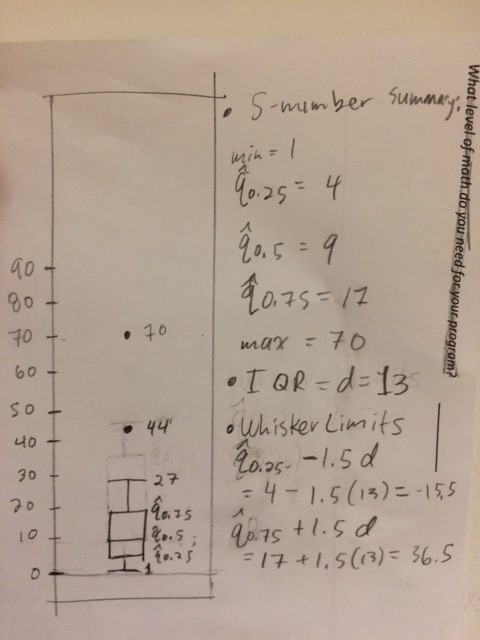
\includegraphics[scale=0.6]{IMG_2605}
\end{center}

The limits of the box are the 1st and 3rd quartile markers, 4 and 17. The bar in the middle of the box is $\hat{q}_{0.5}$. The whiskers limits were calculated to be -15.5 and 36.5. The smallest and largest values in the interval $[-15.5,36.5]$ were 1 and 27. These two numbers are where the whisker bars are made. There are two values outlying these bounds, 44 and 70, which are plotted individually. The distribution is not symmetric. We observe that the data is generally skewed to the right (or upward in the way we created the box plot) by the outliers 70 and 44. We note that the mean of the data is 18, which is nearly double $\hat{q}_{0.5} = 9$. The values less than $\hat{q}_{0.5}$ are much more closely grouped than the values greater than $\hat{q}_{0.5}$.

\vspace{1.5em}

\item List the changes to get from slide 65 to 66 in the slide deck EDA1.pdf and explain how each change improves the visual comparison of the two density estimates.

The Density axes are changed so that the vertical axis of each figure matches the height and formatting style of the other, since the Density markers are at different heights with respect to the data on the first slide. An extra tick is also added so that the data does not exceed the highest density marker. Also the histogram formatting is changed to a box so that both figures enclose their data in a box of the same size- which makes it easier to sense the similarity of the two types of plots. This also eliminates the title from the histogram, which was not needed since it is clearly a histogram and also so that it is not the case that one figure has a title and the other does not. There is some spacing added below the 0 point of the density axis of the histogram, which helps it match the kernel density figure. Similarly to the vertical axis, the horizontal axis of the histogram is changed to match the style of the kernel density estimation figure. This again helps to avoid differences in the formatting so that the focus is on the differences in plotting results. Finally the horizontal axis label is changed to "2012 Citigroup Closing Price" in both figures so that they match and to avoid unnecessary information being included in the figures. 
\vspace{1.5em}

\item Choose a ticker symbol: if your initials are a ticker symbol, use that; otherwise choose a publicly traded company that starts with the same letter as your first name and use its ticker symbol.  Download closing price data for 2012 and recreate the visual display in slide 65.  You may need to adjust the bandwidth of the kernel density estimate if the automatic choice is not good.  The answer should include both the visual display and the R code used to create it. \\

The R code will be provided in separate file so that you may run it on your own machine and see the results. I include the plots here as well, which do match slide 65 exactly except for the fact that citi was not used in my case.

\begin{center}
    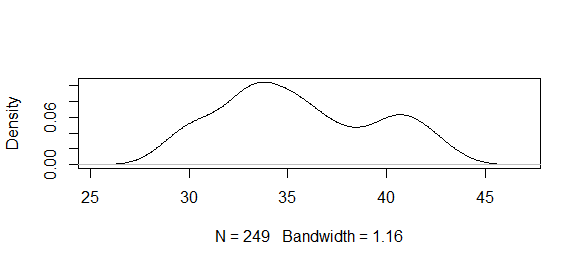
\includegraphics[scale=1]{Rplot}
\end{center}
\begin{center}
    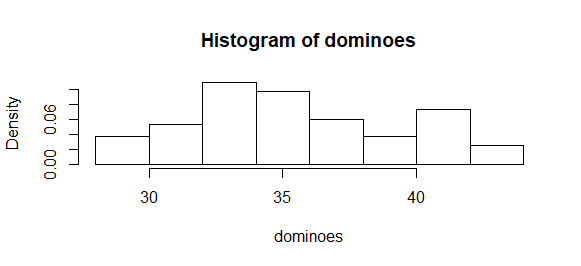
\includegraphics[scale=1]{Rplot01}
\end{center}


\end{enumerate}

\end{document}